\documentclass{article}

\usepackage[margin=0.5in]{geometry}
\usepackage{amsmath}
\usepackage{enumitem}

\usepackage{flushend}
\usepackage{asymptote}

\title{2.4 More Combinatorics Lecture Problems}
\author{}
\date{}

\begin{document}
\maketitle

\begin{enumerate}
    \item How many paths of shortest length are there from A to B traveling along the grid?
    \begin{center}
        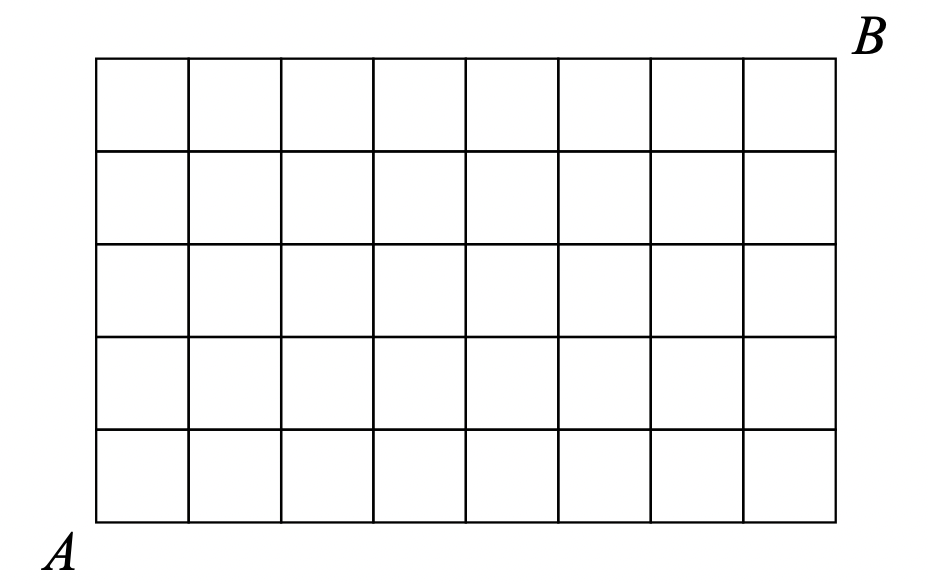
\includegraphics[scale=1]{paths.png}
    \end{center}
        \vspace{3cm}
    \item Alex has ten one-dollar bills to distribute among the five members of 
		Mu Alpha Theta. How many ways are there to distribute his money?
		\vspace{3cm}
	\item How many ways are there to roll a sum of $7$ with three standard 
		six-sided dice?
		\vspace{3cm}
	\item Each of the numbers $1$ through $10$ is placed in a bag and drawn at 
		random with replacement. How many ways can three numbers be drawn whose 
		sum is $13$?
		\vspace{3cm}
\end{enumerate}
\end{document}
